\documentclass[12pt,a4paper]{article}

\usepackage{german}      % Deutsche TeX-Eigenheiten
%\usepackage{isolatin1}   % Eingabekodierung mit Umlauten...

\usepackage{makeidx}
\makeindex            % damit eine Indexdatei angelegt wird

\usepackage{graphicx}

\usepackage{amsmath}  % allgemeine Mathe-Erweiterungen
\usepackage{amssymb}  % Symbole und Schriftarten
\usepackage{amsthm}   % erweiterte Theorem-Umgebungen

\usepackage{mathrsfs}  % gibt den Befehl "\mathscr{}" f�r sch�ne

\begin{document}

\section{21. Die Taylorsche Formel}
Funktion = Summe eines Polynoms + Fehlerterm (Restglied) \\
Problem: Funktionen auf Rechner darstellen ( sin,cos,Expo,..)\\
Grundidee:\\
f(x) durch Polynom Pn(x) approximieren (annähern)\\
Polynom :\\
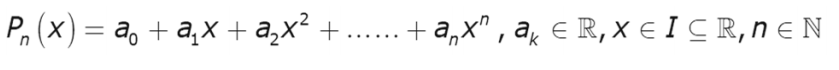
\includegraphics[width=1\textwidth]{BIlder/V1/1.png}
1. Forderung 0 ist im Intervall enthalten\\
Ansatz:\\
Wert von f an der Stelle x (exakt)\\
\= Näherung + Rest\\
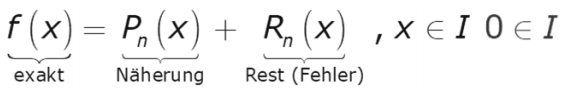
\includegraphics[width=0.5\textwidth]{BIlder/V1/2.png}
\\
Weitere Forderung:\\
an der Stelle 0 soll der Funktionswert und der Wert der k'ten Ableitung von k=0 (0.ableitung)\\
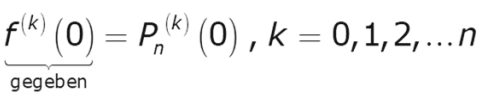
\includegraphics[width=0.4\textwidth]{BIlder/V1/3.png}\\
k'te Ableitung eines Polynoms:\\
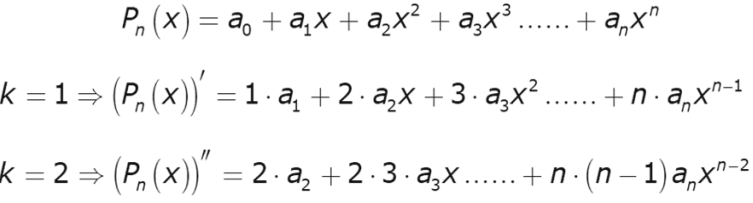
\includegraphics[width=0.5\textwidth]{BIlder/V1/4.png}
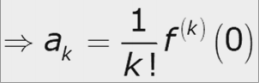
\includegraphics[width=0.3\textwidth]{BIlder/V1/5.png}

\subsection{Näherungspolynom}
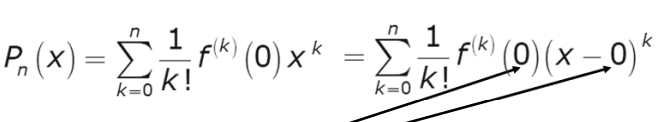
\includegraphics[width=0.5\textwidth]{BIlder/V1/6.png}\\
Stelle 0 geht als Funktionswert ein\\
Wenn x(hoch)k \= (x-0)(hoch)k\\
Problem: 0 nicht im Intervall ?\\
Forderung ist gleich, bzw bezieht sich auf x0\\
= (x-x0)(hoch)k\\
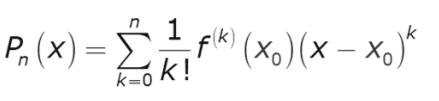
\includegraphics[width=0.4\textwidth]{BIlder/V1/7.png}
\end{document} 

